\renewcommand{\theequation}{\theenumi}
\begin{enumerate}[label=\arabic*.,ref=\thesubsection.\theenumi]
\numberwithin{equation}{enumi}
\item Find the centre and radius of the circle
\begin{equation}
C_1: \vec{x}^T\vec{x} - \myvec{2 & 0}\vec{x} 
-1 = 0 
\label{eq:circle_c1}
\end{equation}
%
\\
\solution let $\vec{c}$ be the centre of the circle.  Then
\begin{align}
\norm{\vec{x}-\vec{c}}^2 &= r^2
\\
\implies \brak{\vec{x}-\vec{c}}^T\brak{\vec{x}-\vec{c}} &= r^2
\\
\implies \vec{x}^T\vec{x} - 2\vec{c}^T\vec{x} &= r^2-\vec{c}^T\vec{c}
\end{align}
%
Comparing with \eqref{eq:circle_c1},
\begin{align}
\vec{c} &= \myvec{1 \\0}
\\
r^2-\vec{c}^T\vec{c} &= 1 \implies r = \sqrt{2}
\end{align}

\item Find the tangent to the circle $C_1$
at the point $\myvec{2 \\1}$.
\\
\solution From \eqref{eq:tangent}, the tangent $T$ is given by
\begin{align}
\sbrak{\myvec{2 & 1}-\myvec{1 & 0}}\vec{x} -\myvec{2 & 1}\myvec{1 \\ 0}  &= 1
\\
\implies T: \vec{n}^T\vec{x}   &= 3
\label{eq:circle_tangent}
\end{align}
%
where
\begin{equation}
\vec{n}=\myvec{1 \\ 1}
\end{equation}
\item The tangent $T$ in \eqref{eq:circle_tangent} cuts off a chord $AB$
from a circle $C_2$ whose 
centre is 
\begin{equation}
\vec{C}=\myvec{3 \\ 
-2}. 
\end{equation}
Find $\vec{A}+ \vec{B}$.
\\
\solution Let the radius of $C_2$ be $r$.  From the given information,
\begin{align}
\brak{\vec{A}-\vec{C}}^T\brak{ \vec{A}-\vec{C} } &= r^2
\label{eq:circle_x1}
\\
\brak{\vec{B}-\vec{C}}^T\brak{ \vec{B}-\vec{C} } &= r^2
\label{eq:circle_x2}
\end{align}
%
 Subtracting 
\eqref{eq:circle_x2} from \eqref{eq:circle_x1},
\begin{flalign}
&\vec{A}^T \vec{A}-\vec{B}^T \vec{B}-2\vec{C}^T\brak{\vec{A}- \vec{B}}  = 0
\\
&\implies \brak{\vec{A}+\vec{B}}^T\brak{ \vec{A}-\vec{B} }-2\vec{C}^T\brak{\vec{A}- \vec{B}} = 0
\nonumber \\
&\implies  \brak{\vec{A}+\vec{B}-2\vec{C}}^T\brak{ \vec{A}-\vec{B} } = 0
\label{eq:circle_aborth}
\end{flalign}
 $\because \vec{A},\vec{B}$ lie on $T$, from \eqref{eq:circle_tangent},
\begin{align}
\label{eq:circle_abtangent}
\vec{n}^T\vec{A} = \vec{n}^T\vec{B}   &= 3
\\
\implies \vec{n}^T\brak{\vec{A} -\vec{B}}   &= 0,
\label{eq:circle_north}
\end{align}
From \eqref{eq:circle_aborth} and \eqref{eq:circle_north}
\begin{align}
\label{eq:circle_abkn}
\vec{A}+\vec{B}-2\vec{C} &= k\vec{n}
\\
\implies \vec{n}^T\vec{A}+\vec{n}^T\vec{B}-2\vec{n}^T\vec{C} &= k\vec{n}^T\vec{n}
\\
\implies \frac{\vec{n}^T\vec{A}+\vec{n}^T\vec{B}-2\vec{n}^T\vec{C}}{\vec{n}^T\vec{n}} &= k
\\
\implies k &= 2
\end{align}
using \eqref{eq:circle_abtangent}.
Substituting in \eqref{eq:circle_abkn}
\begin{align}
\vec{A}+\vec{B} &= 2\brak{\vec{n}+\vec{C}}
\label{eq:circle_a+b}
\end{align}
%
\item If $AB = 4$, find $\vec{A}^T\vec{B}$.
%
\\
\solution From the given information,
\begin{align}
\norm{\vec{A}-\vec{B}}^2 &= 4^2
\end{align}
resulting in
\begin{align}
\norm{\vec{A}+\vec{B}}^2-\norm{\vec{A}-\vec{B}}^2 &= 4\norm{\vec{n}+\vec{C}}^2-4^2
\\
\implies\vec{A}^T\vec{B} &= \norm{\vec{n}+\vec{C}}^2-4 = 17
\end{align}
using \eqref{eq:circle_a+b} and simplifying.
%
\item Show that
\begin{equation}
\label{eq:circle_acb}
\brak{\vec{A}-\vec{C}}^T\brak{\vec{B}-\vec{C}} =8 - r^2
\end{equation}
\\
\solution
\begin{align}
\norm{\vec{A}-\vec{B}}^2 &= 4^2
\\
\implies\brak{\vec{A}-\vec{B}}^T\brak{ \vec{A}-\vec{B} } &= 4^2
\label{eq:circle_x1x2}
\end{align}
%
From \eqref{eq:circle_x1x2},
\begin{align}
\sbrak{\brak{\vec{A}-\vec{C}}-\brak{\vec{B}- \vec{C}}}^T\sbrak{ 
\brak{\vec{A}-\vec{C}}-\brak{\vec{B}- \vec{C}}} = 4^2
\end{align}
%
which can be expressed as
\begin{align}
\norm{\vec{A}-\vec{C}}^2+\norm{\vec{B}-\vec{C}}^2 &
+ 2\brak{\vec{A}-\vec{C}}^T\brak{\vec{B}-\vec{C}} 
= 4^2
\end{align}
Upon substituting from \eqref{eq:circle_x2} and  \eqref{eq:circle_x1} and simplifying, \eqref{eq:circle_acb}
is obtained.
\item Find $r$.
\\
\solution \eqref{eq:circle_acb} can be expressed as
\begin{align}
 \vec{A}^T\vec{B}  -\vec{C}^T\brak{\vec{A}+\vec{B}}+\vec{C}^T\vec{C} &=8 - r^2
\\
\implies 8 - \vec{A}^T\vec{B}  +\vec{C}^T\brak{\vec{A}+\vec{B}}-\vec{C}^T\vec{C} &= r^2
\\
\implies 8 - \vec{A}^T\vec{B}  +\vec{C}^T\brak{2\vec{n}+\vec{C}} &= r^2
\\
\implies r =  \sqrt{6}.
\end{align}
\item Summarize all the above computations through a Python script and plot 
the tangent and circle.
\\
\solution The following code generates Fig. \ref{fig:circle}.
\begin{lstlisting}
wget 
codes/2d/circ.py
\end{lstlisting}
\begin{figure}
\centering
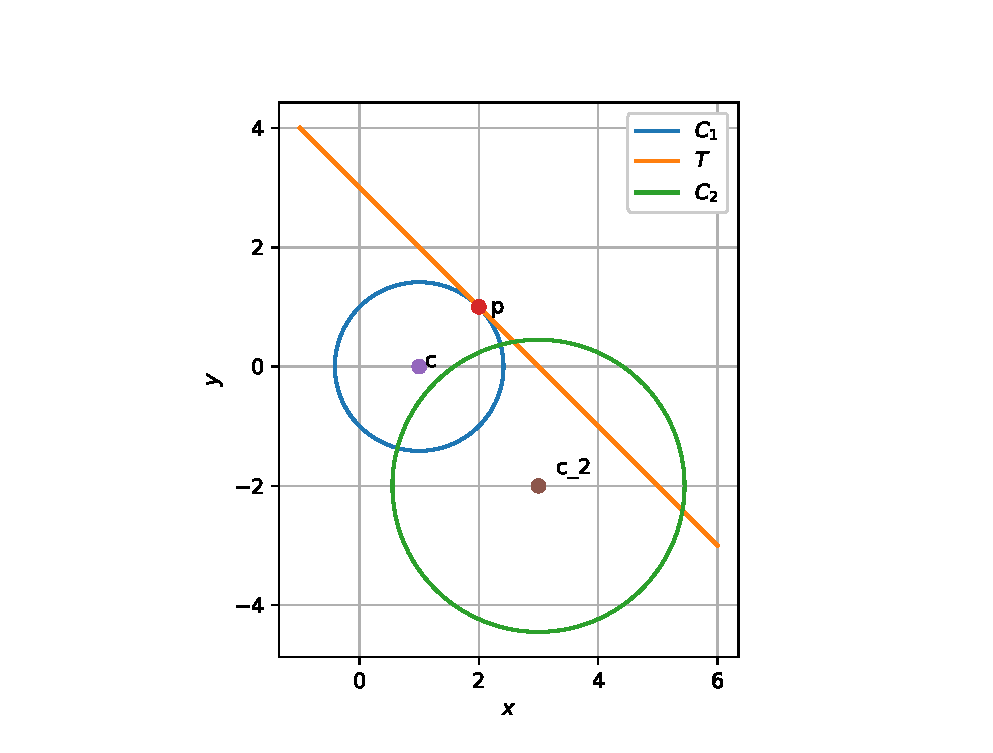
\includegraphics[width=\columnwidth]{./circle/figs/circle.eps}
\caption{}
\label{fig:circle}
\end{figure}

\end{enumerate}


